\documentclass{article}
\usepackage{amsmath}
\usepackage{amssymb}
\usepackage{stmaryrd}
\usepackage{graphicx}
\usepackage{tikz}
\usetikzlibrary{automata, arrows}
\usepackage[ampersand]{easylist}

% needs to be updated
\author{Max Springenberg, 177792}
\title{\
}
\setcounter{section}{1}
\date{}

% custom commands
% \Theta \Omega \omega
\newcommand{\tab}{\null\ \qquad}
\newcommand{\gap}{\null\ \\ \\}
\newcommand{\lA}{$\leftarrow$}
\newcommand{\rA}{$\rightarrow$}
\newcommand{\ue}{$\infty$}
\newcommand{\eps}{$\epsilon$}
\newcommand{\task}[1]{\textbf{#1} \\ \gap}

% content
\begin{document}
% title page
\maketitle
\newpage

% actual paper
\subsection\
\subsubsection{\
    Welche Sprache wird durch den erweiterten regulären Ausdruck ${({ab}^+)}^+$
    über dem Alphabet $\Sigma = \{a,b\}$beschrieben? Wie lautet ein äquivalenter 
    regulärer Ausdruck ohne die in der Vorlesung einge- führte erweiterte 
    Syntax?
    }
der ausdruck ${(ab^+)}^+$ beschreibt die Sprache $L({(ab^+)}^+)$\\
Die durch den Regulaeren Ausdruck beschriebenen Regeln fuer L sind:\\
\begin{easylist}
    & jedes Wort faengt mit einem a an
    & auf jedes a folgt mindestens ein b
    & es muss mindestens ein a und ein b aufeinander folgend vorkommen
\end{easylist}
\ \\
ein aequivalenter Ausdruck fuer ${(ab^+)}^+$ ohne die in der Vorlesung
vorgestellte erweiterte Syntax waere $abb^*{(abb)}^*$, da:$\\
    (abb^* \equiv ab^+) \land (v^+ \equiv vv^* \text{, mit v = } abb^*)\\
    $
\gap\
\subsubsection\

\task{\
    {(a)} Konstruieren Sie einen regulären Ausdruck für die Menge L aller 
    Wörter aus $\{0,1\}$, die ihr erstes Zeichen genau zwei weitere Male, also 
    insgesamt dreimal, enthalten.\\
    Beispiel: $000 \in L, 0010 \in L, 0111010 \in L, 0010011 \in L, \eps \in L$.
    }
Offensichtlich sind moegliche erste Zeichen 0 und 1 oder garkein Zeichen.\\
damit entspricht der Regulaere Ausdruck a, der die Sprache entscheidet, der Form 
$a = (1v + 0u)*$, mit:\\
$v \in \{0,1\}$ als bliebiges Wort, dass mindestens zwei Einsen 
und $u \in \{0, 1\}$ als beliebiges Wort, dass mindestens zwei Nullen enthaelt.\\
Nun bleibt die Form der regulaeren Ausdruecke v und u zu klaeren.\\
Dem Beschriebenem kann entnommen werden, dass eine Analogie im Aufbau der
regulaeren Ausdruecke, die u und v beschreiben existiert.\\
v kann mit 0 und 1 anfangen und vor der ersten 1 darf beliebig oft 0 vorkommen.
Daraus folgt $v = 0^*1v'$, wobei v' wie auch v mit 0 und 1 anfangen kann und vor 
der ersten 1 darf beliebig oft 0 vorkommen. Ferner kann v mit einer beliebigen
Folge aus $\{0, 1\}$ enden.
Daraus folgt $v' = 0^*1{(0^*1*)}^*$ und $v = 0^*1v' = 0^*10^*1{(0^*1^*)}^*$.\\
Da v und u Analog aufgebaut sind kann u mit $u = 1^*0u' = 1^*01^*0{(1^*0^*)}^*$
gebildet werden.\\
Der regulaere Ausdruck a hat damit also die Form:\\
\[
    a = {(1v + 0u)}^*\\
    = {(10^*10^*1{(0^*1^*)}^* + 01^*01^*0{(1^*0^*)}^*)}^*
\]
und es gilt $L = L(a)$\\
\subsubsection\

\task{\
    (b) Passwort p ueber $\Sigma = \{a,\ldots,z,A,\ldots,Z,1,\ldots,9\}$ 
    mit Bedingungen:\\
    (i) Auf keinen Kleinbuchstaben folgt direkt ein Großbuchstabe.\\
    (ii) Auf keinen Großbuchstaben folgt direkt ein Kleinbuchstabe.\\
    (iii) Es ist mindestens eine Ziffer enthalten.\\
    (iv) Das erste Zeichen ist keine Ziffer.
    }
Konvention: Zeichen aus $\Sigma$ seien in drei Gruppen eingeteilt, sodass:\\
\\
$\Sigma \equiv KL \cup GR \cup NUM$\\
, mit $
    KL = \{a,\ldots,z\}
    , GR = \{A,\ldots,Z\}
    , NUM = \{1,\ldots,9\}
    $\\
\\
1. Sprache aller richtigen Passwoerter:\\
Aus {(i)} und {(ii)} folgt der Ausdruck $a = {(k^+n^+g^+ + g^+k^+n^+ + n^*)}^*$, 
    mit $ k \in KL, g \in GR, n \in NUM$\\
\\
Aus {(iii)} und {(iv)} folgt der Ausdruck $b = {(g^+ + k^+)}nw$,
    mit $ k \in KL, g \in GR, n \in NUM$ und w als regulären Ausdruck,
    der {(i)} und {(ii)} erfuellt\\
\\
Somit kann ein legitimes Passwort p durch den regulaeren Ausdruck:\\
\[
    p = ba = {(g^+ + k^+)}n {(k^+n^+g^+ + g^+k^+n^+ + n^*)}^*
\]
formuliert werden.\\
\ \\
2. Sprache aller falschen Passwoerter:\\
Fuer die Sprache aller falschen Passwoerter muessen wir alle Aussagen negieren
und verodern, da bereits eine Regelverletzung zu einem unsicherem Passwort
fuehrt.\\
(i) es existiert ein Kleinbuchstaben, auf den direkt ein Großbuchstabe folgt.\\
(ii) es existiert ein Großbuchstabe, auf den direkt ein Kleinbuchstabe folgt.\\
(iii) Es ist keine Ziffer enthalten.\\
(iv) Das erste Zeichen ist eine Ziffer.
\\
Aus {(i)} folgt der Ausdruck $a_f = \Sigma^*g^+k^+\Sigma^*$,
    mit $ k \in KL, g \in GR, n \in NUM$\\
Aus {(ii)} folgt der Ausdruck $b_f = \Sigma^*k^+g^+\Sigma^*$,
    mit $ k \in KL, g \in GR, n \in NUM$\\
Aus {(iii)} folgt der Ausdruck $c_f = {(g^*k^*)}^*$,
    mit $ k \in KL, g \in GR$\\
Aus {(iv)} folgt der Ausdruck $d_f = n\Sigma^*$,
    mit $n \in NUM$\\
\\
daraus folgt der Ausdruck:\\
\[
    p_f = a_f + b_f + c_f + d_f\\
        = \Sigma^*g^+k^+\Sigma^* 
            + \Sigma^*k^+g^+\Sigma^* 
            + {(g^*k^*)}^* + n\Sigma^*
\]\\
\gap\
\subsection\
\subsubsection{\
    Gegeben sei der folgende DFA\@. Erlaeutern si die Funktion.
    }
\begin{tikzpicture}
    % in Q
    \node[state](q2) at (2,2) {$q_2$};
    \node[state](q1) at (4,0) {$q_1$};
    % in F
    \node[initial, state, accepting, circle, draw=black](q0) at (0,0) {$q_0$};
    % Transitions
    \path
        (q0)
            edge [->, loop below] node {0,3,6,9} (q0)
            edge [->, bend right, top] node {1,4,7} (q1)
            edge [->, bend left, left] node {2,5,8} (q2)
        (q1)
            edge [->] node {2,5,8} (q0)
            edge [->, loop below] node {0,3,6,9} (q1)
            edge [->, bend right, right] node {1,4,7} (q2)
        (q2)
            edge [->] node {2,5,8} (q1)
            edge [->] node {1,4,7} (q0)
            edge [->, loop above] node {0,3,6,9} (q2)
        ;
\end{tikzpicture}
\\
\gap\
Der Automat berechnet ${mod}_3$.\\
\\
Summiert man die modulo-Werte der Ziffern einer Dezimalzahl auf und rechnet
modulo auf dieser Summe erhaelt man das selbe ergebnis, wie wenn man modulo auf
der gesamten Zahl rechnet.\\
Der Automat wechselt fuer jede Ziffer gemaess dem Modulo-Rest dieser Ziffer in
den naechsten Zustand. Dabei wird fuer jede Ziffer x wie im Zustand $q_i$ wie 
folgt vorgegangen:\\
(i) gilt $x \equiv_3 0$ wird im Zustand verweilt\\
(ii) gilt $x \equiv_3 1$ wird in den Zustand $q_{{mod}_3(i+1)}$ gewechselt\\
(iii) gilt $x \equiv_3 2$ wird in den Zustand $q_{{mod}_3(i+2)}$ gewechselt\\
Folglich gilt fuer die TransitionsFunktion:\\
\[
    \delta(q_i, \sigma) = q_{{mod}_3(i+{mod}_3(\sigma))}
\]
\\
Es wird nur im Startzustand $q_0$ akzeptiert. Damit berechnet der Automat
$\mod_3$ korrekt.\\
\gap\
\subsubsection\
\task{
    (a) beschreiben Sie die von dem Automaten beschriebene Sprache
        umgangssprachlich in 1-2 Saetzen.
    }
Der Automat entscheidet Die Sprache $L$ 
ueber das Alphabet $\Sigma = \{0,1\}$, fuer die alle Woerter entweder mit einer
0 beginnen oder eine 0 an einer Stelle $i \in \{2*k | k \in \mathbb{N}\}$ 
enthalten.\\
\\
\task{
    Konstruieren sie einen DFA fuer die Sprache\[
        L = \{w \in \{0,1\}* | w \text{ endet auf zwei gleiche Zeichen}\}
    \]}
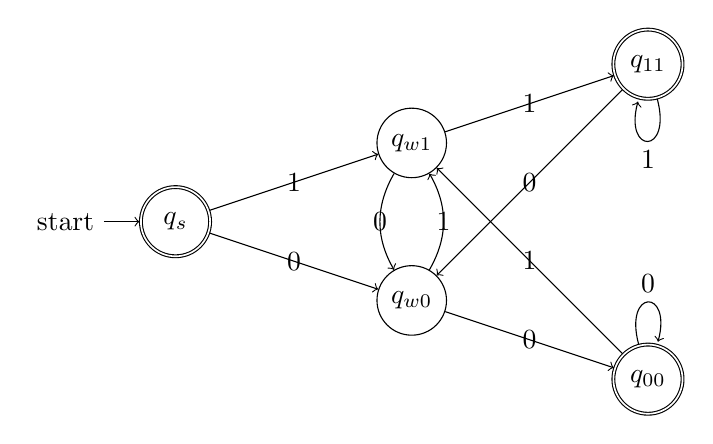
\begin{tikzpicture}
    % in Q
    \node[state](qw1) at (3,2) {$q_{w1}$};
    \node[state](qw0) at (3,0) {$q_{w0}$};
    % in F
    \node[initial, state, accepting, circle, draw=black](qs) at (0,1) {$q_s$};
    \node[state, accepting](q11) at (6,3) {$q_{11}$};
    \node[state, accepting](q00) at (6,-1) {$q_{00}$};
    % Transitions
    \path
        (qs)
            edge [->] node {1} (qw1)
            edge [->] node {0} (qw0)
        (qw0)
            edge [->] node {0} (q00)
            edge [->, bend right] node {1} (qw1)
        (qw1)
            edge [->] node {1} (q11)
            edge [->, bend right] node {0} (qw0)
        (q00)
            edge [->, loop above] node {0} (q00)
            edge [->] node {1} (qw1)
        (q11)
            edge [->, loop below] node {1} (q11)
            edge [->] node {0} (qw0)
        ;
\end{tikzpicture}
\end{document}
